\documentclass{article}
\usepackage{amsmath}
\usepackage{pgfplots}

\begin{document}

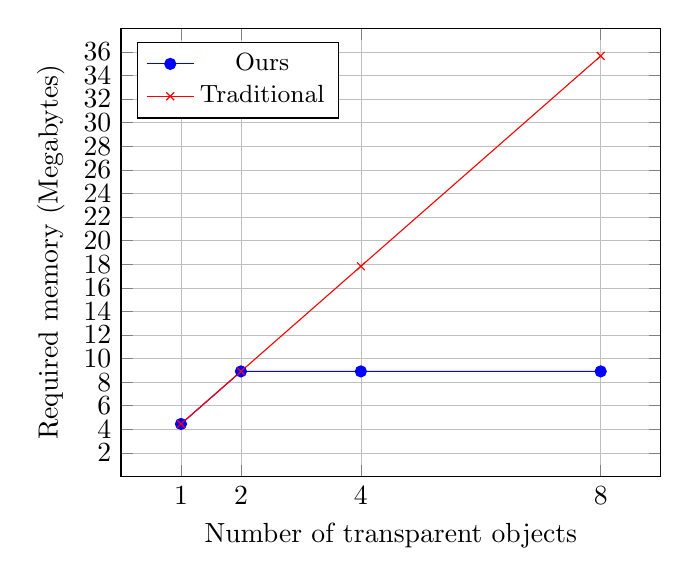
\begin{tikzpicture}
  \begin{axis}[
      xlabel=Number of transparent objects,
      ylabel=Required memory (Megabytes),
      xmin=0, xmax=9,
      ymin=0, ymax=38,
      xtick={1,2,4,8},
      ytick={2, 4, 6, 8, 10, 12, 14, 16, 18, 20, 22, 24, 26, 28, 30, 32, 34, 36},
      legend pos=north west,
      grid=both,
      grid style={line width=.1pt, draw=gray!10},
      major grid style={line width=.2pt,draw=gray!50},
      legend style={font=\small} 
      ]
  \addplot[mark=*,blue] plot coordinates {
      (1,4.456)
      (2,8.912)
      (4,8.912)
      (8,8.912)
  };
  \addlegendentry{Ours}

  \addplot[color=red,mark=x]
      plot coordinates {
        (1,4.456)
        (2,8.912)
        (4,17.824)
        (8,35.648)
      };
  \addlegendentry{Traditional}
  \end{axis}
\end{tikzpicture}

\end{document}